\chapter{Evaluation}\label{ch:results}

The resulting transformation can handle programs where only integer
arithmetic is abstracted. We provide an ability for pointers to point to
abstract values and structures to contain abstract elements. However, we are
currently not able to insert abstract values into arrays, represent abstract
pointers or perform a dynamic memory allocation of abstract values. These
limitations are caused by insufficient representation of abstract
data.\sidenote{Currently, we are not able to represent elements of arrays by
shapes for abstract values. We think this can be easily implemented in a similar
manner as the abstraction of aggregate types. Further limitations represent a
runtime indices into the arrays, which we are not able to compute during
transformation.}For further evaluation we have omitted programs that contain
these unsupported characteristics.

Other technicalities, such as support of threading and support of full \Cpp{}
standard library is inherited from \DIVINE, since transformations do not
interfere with the explicit computation of a program.

To show that the proposed approach is a sufficient replacement of \SymDIVINE, we
will compare the symbolic transformation with \DIVINE as a backend against
\SymDIVINE. Evaluation will be done on the subset of benchmarks from the software
verification competition (\svcomp)~\cite{Beyer17}.
Moreover, to prove the capabilities of the transformation, we will benchmark
verification of basic data structures, specifically binary trees and the more
complicated \AVL tree.

All measurements were performed on machine with 24-core cpu (\code{Xeon E5-2630
v2, 2.60GHz}), and sufficient amount of memory 125 GB.\sidenote{Neither of
benchmarks have reached this bound.} We have restricted benchmarks to use
only four cores.

\section{\textsc{sv-comp} benchmarks}

Out of all \svcomp benchmarks, we have chosen only those that contain
nondeterminism on integers. The rules of \svcomp define a set of builtins for the
verification tool, such as assume, assert and nondeterministic
input~\cite{svcomp}. We have implemen\-ted these intrinsics using the annotations.
For example, the implementation of \code{\_\_VERIFIER\_nondet\_int()} is as
follows:

\begin{minted}{cpp}
int __VERIFIER_nondet_int() {
    _SYM int value;
    return value;
}
\end{minted}
Further specification of the \svcomp builtins can be found in
\autoref{ch:appendixb} or in the competition rules~\cite{svcomp}.

All benchmarks are included in the archive of this thesis. They are further
partitioned into the following categories:
\begin{itemize}
    \item \textbf{pthreads}: programs that contain parallelism,
    \item \textbf{loops}: programs with loops that depends on input value,
    \item \textbf{recursion}: recursive programs taking an arbitrary input,
    \item \textbf{bitvector}: programs that make complex binary operations,
    \item \textbf{product-lines}: generated program modeling products, such as
        elevator,
\end{itemize}

Using those benchmarks, we have compared our implementation to \SymDIVINE. In
particular, we have measured how many benchmarks we were able to verify in a timeframe of 1 hour correctly.

In \autoref{tbl:resultsdiv} and \autoref{tbl:resultssym} we summarize each
category for both tools. We count how many programs were correctly decided to be
valid (\textbf{valid}), in how many benchmarks we have found a reachable error
(\textbf{error}), number of timeouts (\textbf{timeout}) and number of failed
verifications, either caused by an error during the verification (\textbf{unknown})
or reporting a wrong result (\textbf{wrong}).

\begin{table}
  \begin{center}
    \begin{tabularx}{\textwidth}{l r r r r r r }
      \toprule
      & ~ & \multicolumn{5}{c}{\DIVINE + transformation} \\
      \cmidrule(l){3-7}
        & & valid & error & timeout & unknown & wrong \\
      \midrule
        pthreads &        & $0$ & $1$  & $4$ & $0$  & $1$ \\
        loops &           & $4$ & $14$ & $5$ & $0$  & $0$ \\
        recursion &       & $4$ & $15$ & $18$ & $3$  & $0$ \\
        bitvector &       & $7$ & $2$  & $16$ & $2$  & $0$ \\
        product-lines &   & $2$ & $6$  & $2$  & $0$  & $0$ \\
      \midrule
      \midrule
        overall &         & $17$ & $38$ & $45$ & $5$ & $1$ \\
      \bottomrule
    \end{tabularx}
  \end{center}
  \caption{Evaluation of \DIVINE with transformation on \svcomp benchmarks.}
  \label{tbl:resultsdiv}
\end{table}
\begin{table}
  \begin{center}
    \begin{tabularx}{\textwidth}{l r r r r r r }
      \toprule
      & ~ & \multicolumn{5}{c}{\SymDIVINE} \\
      \cmidrule(l){3-7}
        & & valid & error & timeout & unknown & wrong \\
      \midrule
        pthreads &        & $0$ & $1$  & $4$  & $0$ & $1$ \\
        loops &           & $6$ & $11$ & $4$  & $0$ & $2$ \\
        recursion &       & $2$ & $11$ & $27$ & $0$ & $0$ \\
        bitvector &       & $6$ & $4$  & $17$ & $0$ & $0$ \\
        product-lines &   & $3$ & $7$  & $0$  & $0$ & $0$ \\
      \midrule
      \midrule
        overall &         & $17$ & $34$ & $52$ & $0$ & $3$ \\
      \bottomrule
    \end{tabularx}
  \end{center}
  \caption{Evaluation of \SymDIVINE on \svcomp benchmarks.}
  \label{tbl:resultssym}
\end{table}

Results show that \DIVINE with transformation performs slightly better than
\SymDIVINE. Besides completed verification and timeouts, we got $5$ unknown
results caused by a failure during the verification. Moreover, \DIVINE decided
one benchmark wrongly; we believe that this benchmark is falsely marked as
valid, because both \SymDIVINE and \DIVINE found an error in it.

In all benchmarks, the transformation successfully finishes in a few seconds.
But differences between tools have shown during the verification. Surprisingly
\SymDIVINE competes with \DIVINE quite well. Why is it so?

Even though \DIVINE utilizes $\tau$-reduction and a faster \LLVM interpreter,
the bottleneck of verification is the interface with an \SMT solver. For each
\SMT query \DIVINE spawns a new process with a solver, and that requires a nontrivial amount of time. Moreover, communication with the solver is
performed inefficiently, via a string stream.

In \SymDIVINE, the process running the \SMT solver is maintained during the
entire course of verification, hence it saves time on process creation.
Moreover, the communication with the solver is via a dedicated interface,
which is faster. Additionally, \SymDIVINE utilises caching of queries.
Hence, \SymDIVINE can explore a state-space much faster (around 200 states
per second), but it encounters larger state spaces, because of missing state
space reductions. On the other hand, \DIVINE proceeds more slowly (around 10
states per second), but profits from smaller state spaces.

For comparison, we attach a quantitative plot of solved benchmarks by both tools
in the \autoref{fig:accu}.
Most of the benchmarks are solved in a matter of seconds by both tools, but with
higher timeframe, \DIVINE solve slightly more of them.

\begin{figure}
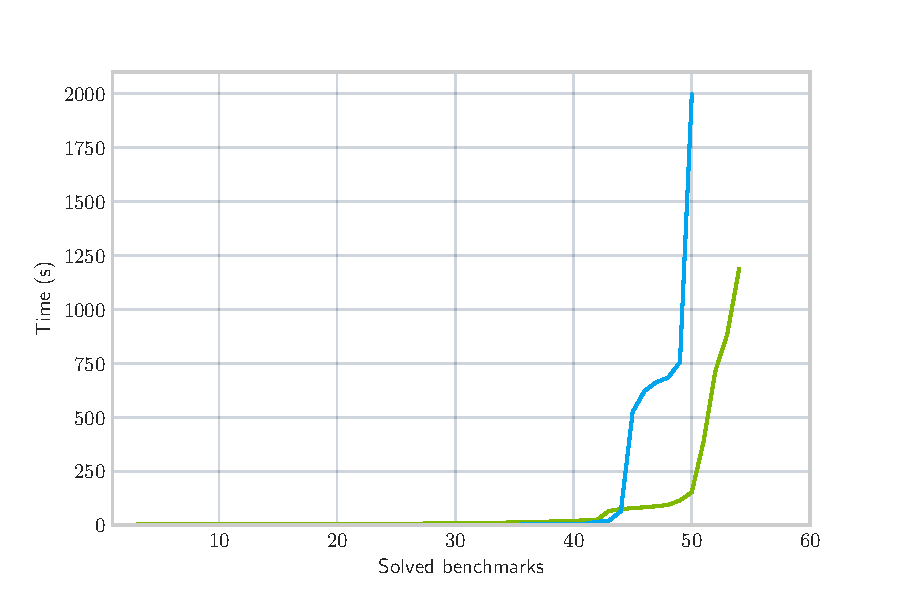
\includegraphics[width=\textwidth]{img/accum.pdf}
    \caption{A comparison of \DIVINE (green) and \SymDIVINE (blue).}
    \label{fig:accu}
\end{figure}
Further, we made a comparison of state space sizes (\autoref{fig:ss}). In this case, \SymDIVINE
surprisingly competes well on the smaller benchmarks (less then 100 state), but
on the larger state spaces \DIVINE has significantly better results.

\begin{figure}
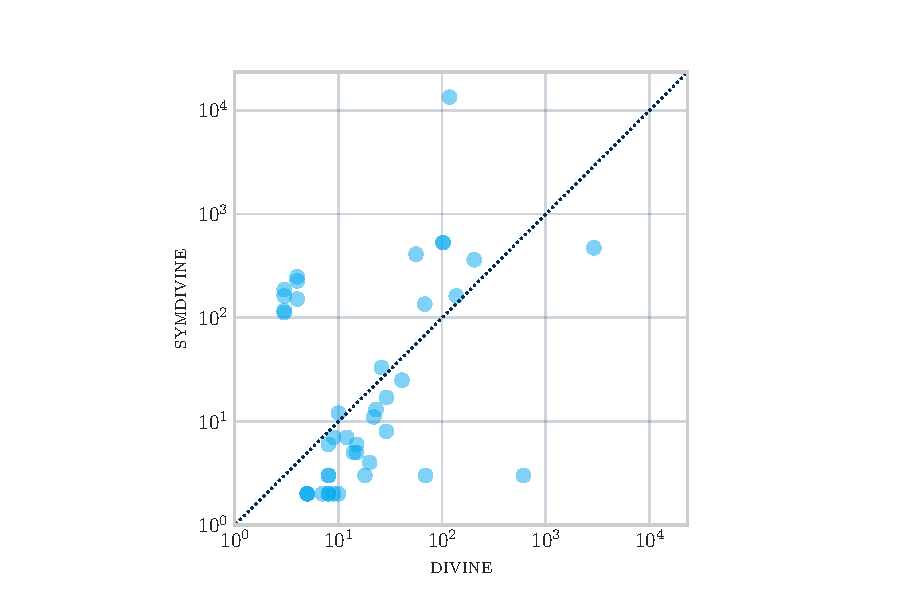
\includegraphics[width=\textwidth]{img/scatter.pdf}
    \caption{A comparison of \DIVINE and \SymDIVINE state space sizes.}
    \label{fig:ss}
\end{figure}

Complete results can be found in the thesis archive. Here we have summarised
only the significant data.

\section{Data structures}

The data structure benchmarks show the most significant contribution of a symbolic
approach. By the symbolic representation of elements in data structures, we can
verify all possible behaviours for a given number of inputs. In these
benchmarks, we demonstrate how much time the transformation takes and how
much time \DIVINE spends in the verification process. We do not provide a
comparison with \SymDIVINE because it is unable to verify this type of
programs.

In all these benchmarks, we try to verify insertions and deletions of arbitrary
values from the data structures. The data structures are stored on the
stack because we are limited in transformation by dynamic memory allocation.
We use the following naming convention for the benchmarks: \code{\{name\}-\{num. of
insertion\}-\{num. of deletions\}-\{V/E for validity or an\\error\}}.

\begin{table}[!h]
  \begin{center}
    \begin{tabularx}{\textwidth}{l r r r}
      \toprule
      Benchmark Name & Transformation & Verification & States \\
        \midrule
        \code{sorted-list-3-0-V} & $2.10s$ & $37s$ & $39$ \\
        \code{sorted-list-4-0-V} & $2.62s$ & $2m 14s$ & $155$ \\
        \code{sorted-list-5-0-V} & $2.04s$ & $8m 15s$ & $733$ \\
        \code{sorted-list-3-0-E} & $2.29s$ & $0.02s$ & $14$ \\
        \code{sorted-list-4-0-E} & $2.17s$ & $58s$ & $31$ \\
        \code{sorted-list-5-0-E} & $2.05s$ & $2m 57s$ & $57$ \\
        \midrule

        \code{bintree-3-0-V} & $2.23s$ & $7s$ & $78$ \\
        \code{bintree-4-0-V} & $2.77s$ & $1m 14s$ & $332$ \\
        \code{bintree-5-0-V} & $3.22s$ & $4m 12s$ & $1846$ \\
        \code{bintree-3-1-V} & $4.54s$ & $11.8s$ & $124$ \\
        \code{bintree-3-2-V} & $3.91s$ & $22.3s$ & $168$ \\
        \code{bintree-3-3-V} & $3.44s$ & $12.9s$ & $195$ \\

        \midrule

        \code{avl-1-0-V} & $2.96s$ & $1.93s$ & $16$ \\
        \code{avl-2-0-V} & $3.11s$ & $8.31s$ & $64$ \\
        \code{avl-3-0-V} & $2.87s$ & $39s$ & $346$ \\
        \code{avl-4-0-V} & $3.06s$ & $3m~27s$ & $1464$ \\
        \code{avl-5-0-V} & $2.98s$ & $14m~16s$ & $9242$ \\
      \bottomrule
    \end{tabularx}
  \end{center}
  \caption{Benchmarks of insertions and deletions from the data
    structures. A~name of benchmark represents a data structure, number of insertions and number of deletions. \code{V} or \code{E} at the end of
    the name denotes whether the benchmark is valid or contains an error.}
\end{table}

From the results, we can see that the bottleneck is still verification. Even though,
we have defeated data nondeterminism; we have introduced a lot of control flow
nondeterminism because of nondeterministic choices on branches. The transformation
time is approximately 10 seconds. The average speed of verification is two states
per second. We believe that this is a consequence of the slow \API between the model
checker and the \SMT solver, since \SymDIVINE was able to generate 200 states
per seconds in an average, with a less optimized exploration algorithm. Hence we
believe that in the future, we can optimize the search algorithm to cope with
larger state spaces in a reasonable time.

In benchmarks of the \AVL tree, we can see that despite the increasing number of
inputs, the transformation time stays the same, but the verification time
exponentially grows. The exponential growth is caused by the nature of the \AVL
tree. When we are inserting an arbitrary value, we have to branch the state space
on each comparison of the inserted value and node into which we are inserting.
Branching creates two possibilities, first when the value is inserted into the
left subtree and second for the right subtree. This way, we create during a
verification all possible shapes of the \AVL tree for a given number of elements.
A similar phenomenon appears in other data structures, where the algorithm
branches depending on the inserted value.

But since the algorithms on these data structures are simple, most of the errors
are shallow and can be found quickly. Note, for instance, the difference of time
in benchmarks \code{sorted-list\\-3-0-V} and \code{sorted-list-3-0-E}.

During the evaluation, we have appreciated the qualities of the proposed
approach, because besides the verification of the program we have verified the
implementation of the abstraction and fixed minor bugs that we have found. This
would have been much harder if the abstraction would be implemented inside of the
verification tool.
